The first part of our all-atom fitting algorithm is to fit the protein backbone to the given \Ca-trace ignoring the side-chain conformations.

As input we are given a \Ca-trace target and a protein in form of an amino acid sequence.
Only the amino acid types are provided; no spatial structure information about the protein is given as this is left to the fitting algorithm to find.


\section{Limitations}
The adjustable parameters in a protein backbone structure consists of bond angles, dihedral angles and bond lengths.
As the dihedral angles are by far the most influential parameters we allow ourselves to perform the simplification of not considering bond lengths and bond angles.
More specifically, we will only adjust the $\phi$ and $\psi$ angles on the atom bonds between \Ca-C and \Ca-N.
For all other parameters we use known constants that approximate the average backbone structure.
Thus, the protein backbone to be folded becomes a sequence of identical amino acid backbones that can only be modified by adjusting $\phi$ and $\psi$ for each amino acid.


\section{Inverse kinematics}
With the above limitations in place the backbone fitting problem can be regarded as an \emph{inverse kinematics} (IK) problem.
IK is the process of determining angles of joints in a chain of rigid links in order to make the end of the linked chain reach a desired position in space.
The end of the the linked chain is called the \emph{end-effector}.

In our case, the spatial structure consists of a series of atoms (joints) connected by atom bonds (links).
Our backbone fitting problem is not an ordinary IK problem since we have multiple end-effectors in form of the target \Ca-trace.

To simplify the problem, we can separately consider each backbone \Ca as an end-effector that must reach its corresponding target \Ca.
In this way the problem is decomposed into many small IK problems.
However, this simplification is not entirely valid as the entire backbone cannot be fitted by solving many local problems.
For example, a configuration of $\phi$ and $\psi$ angles might fit a single \Ca well to its target, but in such a way that the next \Ca in the backbone cannot come close to its target.
Therefore, a good solution should take global context into account when solving IK problems locally. 

An IK problem may have multiple solutions depending on the number of degrees of freedom (DOF) given by the adjustable angles.
In our fitting problem, we just want a single solution.
In most cases, however, there is no solution as our limitations make it impossible to conform to a given \Ca-trace.
Furthermore, it is possible that the given \Ca-traces have a completely unrealistic structure.
In these cases, we just want a solution that is somewhat close to the target.

%As we have decided not to consider the bond angles (joint angles), the only adjustable angles in the kinematic chain are the dihedral angles around the atom bonds between \Ca-C and \Ca-N.
%\fxfatal{skal vi indsætte en simpel IK-illustration her?} 

\subsection{Related work}
Several IK solving methods exist and have been utilized in protein structure prediction.
However, these methods are mainly concerning the \emph{loop closure} problem \cite{coutsias2004kinematic} which differs from our problem since the goal is to fit a single amino acid to a target by adjusting angles in a chain of several residues (typically between 4 and 14).
  
\cite{shenkin1987} describes a Jacobian solution in which the partial derivatives model the movement of the end of the kinematic chain relative to the angular changes.
To calculate the necessary angular changes the Jacobian is simply inverted.
The method then works iteratively by calculating the angular changes and adjusting the angles correspondingly in each step in order to move the end effector towards its target.
%Moreover, the method is capable of handling lower limit constraints on interatomic distances between the end.
This method has one downside according to \cite{canutescu2003}.
If the Jacobian matrix is close to singular by coincidence, the inversion is ill posed yielding unstable results.

Instead, \cite{canutescu2003} proposes a \emph{cyclic coordinate descent} (CCD) method.
CCD decomposes the problem by solving one angle at a time wrt. the end-effector.
1 DOF problems are simple and can be solved analytically.
This is done repeatedly up the link chain, making the end-effector position converge towards the target.
To give more realistic results, a Ramachandran probability map is used to determine if a proposed angle is acceptable. 
It is claimed that their method has very fast performance. 
However, the algorithm may fail to find solutions for short amino acid sequences.
In \cite{boomsma2005full}, the CCD method is extended to include bond angles.

Finally, \cite{wedemeyer1999exact} has proposed a method for solving loop closures with 3 amino acides (6 DOFs) in closed form by reducing the problem to extracting roots of a polynomial.


\section{Our solution}
The backbone fitting problem is different from the loop closure problem as the end-effector covers the entire backbone.
Therefore, the methods above cannot be applied directly to our problem.
As discussed, we must take the global solution into consideration when solving a local IK problem.

We have chosen to experiment with the CCD approach as it is simple, fast, numerically stable, and flexible (ie. it is easy to introduce algorithmic constraints).

\subsection{Cyclic coordinate descent}


\subsection{Results}

%We begin from one end of the amino acid sequence by placing the first two amino acids such that they match the beginning of the \Ca-trace target.


%$||N - C|| \rotateAround{180^\circ} \rotateAround{90^\circ} \rotateAround{v}$

\begin{figure}
  \centering
	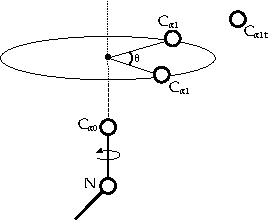
\includegraphics[width=0.75\columnwidth]{figures/ccd_angles}
	\label{fig:ccd_angles}
  \caption{}
\end{figure}

